% !TEX program = pdflatex
\documentclass[aspectratio=169, 11pt]{beamer}

% ============================================================
%  THEME & COLORS
% ============================================================
\usetheme{default}
\usecolortheme{default}
\setbeamertemplate{navigation symbols}{}
\setbeamertemplate{footline}[frame number]

% Custom palette
\definecolor{qDark}{HTML}{1B1F3B}
\definecolor{qBlue}{HTML}{3A86FF}
\definecolor{qCyan}{HTML}{00B4D8}
\definecolor{qAccent}{HTML}{FF006E}
\definecolor{qGray}{HTML}{F0F1F5}
\definecolor{qText}{HTML}{2B2D42}

\setbeamercolor{structure}{fg=qBlue}
\setbeamercolor{frametitle}{fg=white, bg=qDark}
\setbeamercolor{title}{fg=white}
\setbeamercolor{subtitle}{fg=qCyan}
\setbeamercolor{author}{fg=white}
\setbeamercolor{date}{fg=qCyan}
\setbeamercolor{normal text}{fg=qText}
\setbeamercolor{block title}{fg=white, bg=qBlue}
\setbeamercolor{block body}{bg=qGray}
\setbeamercolor{alerted text}{fg=qAccent}
\setbeamercolor{itemize item}{fg=qBlue}
\setbeamercolor{itemize subitem}{fg=qCyan}
\setbeamercolor{footnote}{fg=qText!60}

% Frametitle styling
\setbeamertemplate{frametitle}{%
  \nointerlineskip
  \begin{beamercolorbox}[wd=\paperwidth, ht=2.8em, dp=1em, leftskip=1.2em]{frametitle}%
    \usebeamerfont{frametitle}\insertframetitle
  \end{beamercolorbox}%
}

% Title page background
\setbeamertemplate{title page}{%
  \begin{tikzpicture}[remember picture, overlay]
    \fill[qDark] (current page.north west) rectangle (current page.south east);
    \foreach \i in {1,...,40}{%
      \pgfmathsetmacro{\x}{rnd*16}
      \pgfmathsetmacro{\y}{rnd*9}
      \pgfmathsetmacro{\r}{0.02+rnd*0.06}
      \fill[qBlue, opacity=0.12] (\x, \y) circle (\r);
    }
    \foreach \i in {1,...,15}{%
      \pgfmathsetmacro{\xa}{rnd*16}
      \pgfmathsetmacro{\ya}{rnd*9}
      \pgfmathsetmacro{\xb}{\xa+rnd*3}
      \pgfmathsetmacro{\yb}{\ya+rnd*2}
      \draw[qCyan, opacity=0.08, line width=0.3pt] (\xa, \ya) -- (\xb, \yb);
    }
  \end{tikzpicture}
  \vfill
  \begin{center}
    {\usebeamerfont{title}\usebeamercolor[fg]{title}\LARGE\textbf{\inserttitle}\par}
    \vskip 0.6em
    {\usebeamerfont{subtitle}\usebeamercolor[fg]{subtitle}\large\insertsubtitle\par}
    \vskip 1.5em
    {\usebeamerfont{author}\usebeamercolor[fg]{author}\insertauthor\par}
    \vskip 0.4em
    {\usebeamerfont{date}\usebeamercolor[fg]{date}\small\insertdate\par}
  \end{center}
  \vfill
}

% Fonts
\usefonttheme{professionalfonts}
\setbeamerfont{frametitle}{size=\large, series=\bfseries}
\setbeamerfont{title}{size=\Large, series=\bfseries}
\setbeamerfont{footnote}{size=\tiny}

% ============================================================
%  PACKAGES
% ============================================================
\usepackage[utf8]{inputenc}
\usepackage[T1]{fontenc}
\usepackage{lmodern}
\usepackage{amsmath, amssymb, amsfonts}
\usepackage{physics}
\usepackage{graphicx}
\graphicspath{{figures/simulation/}{figures/analysis/}{simulation/}{analysis/}{./}}
\usepackage{tikz}
\usetikzlibrary{positioning, arrows.meta, calc, decorations.pathmorphing}
\usepackage{booktabs}
\usepackage{appendixnumberbeamer}

% Math shortcuts
\newcommand{\phiplus}{\ket{\Phi^+}}
\newcommand{\pw}{p_{\mathrm{w}}}
\newcommand{\ps}{p_{\mathrm{s}}}

% ============================================================
%  METADATA
% ============================================================
\title{Entanglement Swapping \\ in Quantum Repeater Chains}
\subtitle{Monte Carlo Simulation with QuantumSavory.jl}
\author{Andrea Gennari}
\date{A.Y.\ 2025/2026, Quantum Computing}

\begin{document}

% ============================================================
%  TITLE
% ============================================================
\begin{frame}[plain, noframenumbering]
  \titlepage
\end{frame}

% ============================================================
%  OUTLINE
% ============================================================
\begin{frame}{Outline}
  \begin{columns}[T]
    \begin{column}{0.48\textwidth}
      \textbf{\textcolor{qBlue}{Theory}}
      \begin{enumerate}
        \item Motivation and quantum repeaters
        \item Entanglement swapping protocol
        \item Noise model: depolarization
      \end{enumerate}
    \end{column}
    \begin{column}{0.48\textwidth}
      \textbf{\textcolor{qCyan}{Simulation \& Results}}
      \begin{enumerate}\setcounter{enumi}{3}
        \item Simulator architecture
        \item Ideal case validation
        \item Monte Carlo simulation
        \item Numerical vs.\ theoretical comparison
        \item Emergent effects and conclusions
      \end{enumerate}
    \end{column}
  \end{columns}
\end{frame}

% ============================================================
%  MOTIVATION
% ============================================================
\begin{frame}{Why Quantum Repeaters?}
  \begin{columns}[c]
    \begin{column}{0.55\textwidth}
      \begin{itemize}
        \item Optical fiber: \alert{exponential losses} with distance
        \item \textbf{No-cloning theorem}: no classical amplification
        \item \textbf{Quantum repeaters}: hop-by-hop entanglement distribution
      \end{itemize}
      \vskip 1em
      \begin{block}{Project Goal}
        Simulate Alice$\leftrightarrow$Bob entanglement across $N$ repeaters,
        measuring \textbf{fidelity} and \textbf{distribution time} vs noise.
      \end{block}
    \end{column}
    \begin{column}{0.42\textwidth}
      \centering
      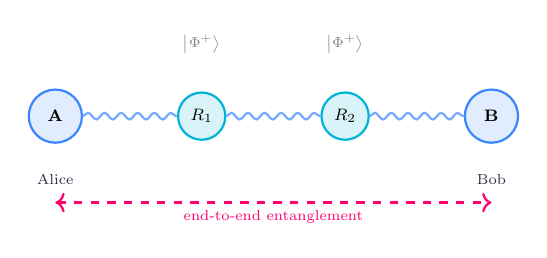
\begin{tikzpicture}[
        scale=0.75, every node/.style={scale=0.75},
        node distance=1.2cm,
        qnode/.style={circle, draw=qBlue, fill=qBlue!15, thick,
                      minimum size=0.9cm, font=\footnotesize\bfseries},
        rep/.style={circle, draw=qCyan, fill=qCyan!15, thick,
                    minimum size=0.8cm, font=\footnotesize\bfseries},
        link/.style={thick, decorate,
                     decoration={snake, amplitude=1.2pt, segment length=6pt},
                     qBlue!70}
      ]
        \node[qnode] (A) {A};
        \node[rep, right=of A] (R1) {$R_1$};
        \node[rep, right=of R1] (R2) {$R_2$};
        \node[qnode, right=of R2] (B) {B};

        \draw[link] (A) -- (R1);
        \draw[link] (R1) -- (R2);
        \draw[link] (R2) -- (B);

        \node[below=0.3cm of A, font=\scriptsize, qText] {Alice};
        \node[below=0.3cm of B, font=\scriptsize, qText] {Bob};
        \node[above=0.4cm of R1, font=\scriptsize, qText!60] {$\phiplus$};
        \node[above=0.4cm of R2, font=\scriptsize, qText!60] {$\phiplus$};

        \draw[qAccent, thick, dashed, <->]
          ([yshift=-1cm]A.south) -- ([yshift=-1cm]B.south)
          node[midway, below, font=\scriptsize] {end-to-end entanglement};
      \end{tikzpicture}
    \end{column}
  \end{columns}
\end{frame}

% ============================================================
%  ENTANGLEMENT SWAPPING PROTOCOL
% ============================================================
\begin{frame}{The Protocol: Entanglement Swapping}
  \begin{columns}[c]
    \begin{column}{0.52\textwidth}
      \textbf{Key idea:} a BSM at the repeater
      teleports entanglement to the remote nodes.

      \vskip 0.8em
      \textbf{For each repeater $R_k$ (a parallel process):}
      \begin{enumerate}
        \item Holds two qubits entangled with left and right neighbours
        \item \textbf{Local BSM} on its two qubits \emph{only}
        \item Sends the 2-bit outcome over a \textbf{classical channel}
        \item Remote node applies the \textbf{Pauli correction} $\to \phiplus$
      \end{enumerate}

      \vskip 0.6em
      The $N$ repeaters swap \textbf{independently}; entanglement extends outward until Alice and Bob share $\phiplus$.
    \end{column}
    \begin{column}{0.45\textwidth}
      \centering
      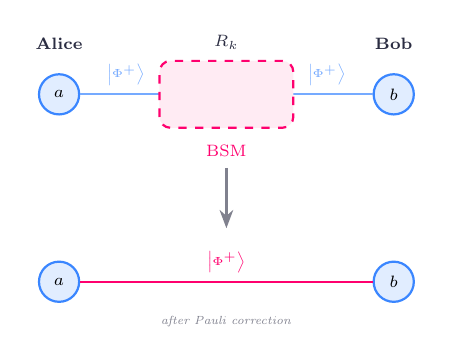
\begin{tikzpicture}[
        scale=0.85, every node/.style={scale=0.85},
        slot/.style={circle, draw, thick, minimum size=0.6cm, font=\scriptsize},
        slotA/.style={slot, draw=qBlue, fill=qBlue!15},
        slotR/.style={slot, draw=qCyan, fill=qCyan!15},
        slotB/.style={slot, draw=qBlue, fill=qBlue!15},
        ep/.style={thick, qBlue!70},
        bsm/.style={draw=qAccent, thick, dashed, rounded corners=4pt}
      ]
        % Nodes
        \node[slotA] (a1) at (0, 2) {$a$};
        \node[slotR] (r1) at (2, 2) {$\ell$};
        \node[slotR] (r2) at (3, 2) {$r$};
        \node[slotB] (b1) at (5, 2) {$b$};

        % Labels
        \node[above=0.2cm of a1, font=\scriptsize\bfseries, qText] {Alice};
        \node[above=0.2cm of r1, font=\scriptsize\bfseries, qText, xshift=0.5cm] {$R_k$};
        \node[above=0.2cm of b1, font=\scriptsize\bfseries, qText] {Bob};

        % Entanglement links
        \draw[ep] (a1) -- (r1) node[midway, above, font=\tiny] {$\phiplus$};
        \draw[ep] (r2) -- (b1) node[midway, above, font=\tiny] {$\phiplus$};

        % BSM box
        \draw[bsm, fill=qAccent!8] ($(r1)+(-0.5,-0.5)$) rectangle ($(r2)+(0.5,0.5)$);
        \node[font=\scriptsize, qAccent] at (2.5, 1.15) {BSM};

        % Arrow to result
        \draw[-{Stealth}, thick, qText!60] (2.5, 0.9) -- (2.5, 0);

        % After swap
        \node[slotA] (a2) at (0, -0.8) {$a$};
        \node[slotB] (b2) at (5, -0.8) {$b$};
        \draw[ep, qAccent] (a2) -- (b2) node[midway, above, font=\tiny] {$\phiplus$};
        \node[font=\tiny, qText!60] at (2.5, -1.4) {\textit{after Pauli correction}};
      \end{tikzpicture}
    \end{column}
  \end{columns}
\end{frame}

% ============================================================
%  NOISE MODEL
% ============================================================
\begin{frame}{Noise Model: Depolarization}
  \begin{columns}[c]
    \begin{column}{0.50\textwidth}
      Quantum memories \textbf{depolarize} while waiting.

      \vskip 0.2em
      {\small Single-qubit depolarizing channel (QuantumSavory convention):}
      \vspace{-0.3em}
      \[
        \mathcal{E}(\rho) = (1 - p)\,\rho + p\,\frac{I}{2}
      \]

      \vspace{-0.4em}
      {\small Noise tied to waiting time:}
      \vspace{-0.3em}
      \[
        p(\Delta t) = 1 - e^{-\Delta t / \tau}
      \]

      \vspace{-0.4em}
      {\small $\tau = -1/\ln(1 - \pw)$, \; $\pw$ = per-step depolarization rate.}

      \vskip 0.25em
      {\small \textbf{Fidelity:}\;
      $F = \tfrac{1}{4}\!\bigl(1 + \expval{XX} + \expval{ZZ} - \expval{YY}\bigr)$}
    \end{column}
    \begin{column}{0.46\textwidth}
      \begin{block}{Why Time Matters}
        {\small If $\ps < 1$, links become ready at different times; the
        end-to-end pair is delivered when the \textbf{slowest} link arrives.}
        \vspace{-0.3em}
        \[
          T = \max_{i=1}^{N+1} T_i, \quad T_i \sim \mathrm{Geom}(\ps)
        \]
        \vspace{-0.3em}
        {\footnotesize Each repeater swaps \textbf{as soon as} it holds both
        halves (at the $\max$ of its two links), so internal qubits are measured
        early and decohere \emph{less}; only Alice's and Bob's qubits wait until
        $T$. This asynchronous schedule is what the discrete-event simulator runs.}
      \end{block}
    \end{column}
  \end{columns}
\end{frame}

% ============================================================
%  ARCHITECTURE
% ============================================================
\begin{frame}{Simulator Architecture}
  \begin{columns}[c]
    \begin{column}{0.45\textwidth}
      \textbf{Language:} Julia \quad
      \textbf{Framework:} QuantumSavory.jl

      \vskip 0.8em
      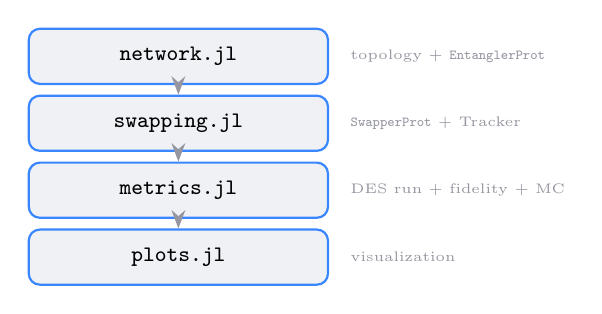
\begin{tikzpicture}[
        box/.style={draw=qBlue, thick, rounded corners=4pt,
                    fill=qGray, minimum width=3.8cm, minimum height=0.7cm,
                    font=\footnotesize},
        arr/.style={-{Stealth}, thick, qText!50}
      ]
        \node[box] (net) at (0, 2.6) {\texttt{network.jl}};
        \node[box] (sw)  at (0, 1.75) {\texttt{swapping.jl}};
        \node[box] (me)  at (0, 0.9) {\texttt{metrics.jl}};
        \node[box] (pl)  at (0, 0.05) {\texttt{plots.jl}};

        \draw[arr] (net) -- (sw);
        \draw[arr] (sw) -- (me);
        \draw[arr] (me) -- (pl);

        \node[font=\tiny, qText!50, right=0.15cm of net] {topology + \texttt{EntanglerProt}};
        \node[font=\tiny, qText!50, right=0.15cm of sw] {\texttt{SwapperProt} + Tracker};
        \node[font=\tiny, qText!50, right=0.15cm of me] {DES run + fidelity + MC};
        \node[font=\tiny, qText!50, right=0.15cm of pl] {visualization};
      \end{tikzpicture}
    \end{column}
    \begin{column}{0.52\textwidth}
      \begin{block}{Linear network: Alice + $N$ repeaters + Bob}
        \vspace{-0.3em}
        {\small
        \begin{itemize}\itemsep0em
          \item Alice/Bob: 1 slot; each repeater: 2 slots
          \item Linear \texttt{RegisterNet} + classical channels
        \end{itemize}}
        \vspace{-0.3em}
      \end{block}

      \vskip 0.2em
      \begin{block}{Discrete-event engine (\texttt{ConcurrentSim} + \texttt{ProtocolZoo})}
        \vspace{-0.3em}
        {\small Parallel \texttt{@resumable} entities on one simulation clock:}
        \vspace{-0.3em}
        {\footnotesize
        \begin{itemize}\itemsep0em
          \item \texttt{EntanglerProt}: heralded Bell-pair generation per link
          \item \texttt{SwapperProt}: asynchronous local BSM at each repeater
          \item \texttt{EntanglementTracker}: classical messages + Pauli corrections
          \item detector process: stops at delivery, measures $F$ and $T$
        \end{itemize}}
        \vspace{-0.3em}
      \end{block}
    \end{column}
  \end{columns}
\end{frame}

% ============================================================
%  PHASE 1: IDEAL VALIDATION
% ============================================================
\begin{frame}{Ideal Case Validation}
  \begin{columns}[c]
    \begin{column}{0.48\textwidth}
      \textbf{Test:} no noise ($\pw = 0$), deterministic ($\ps = 1$)
      $\Rightarrow$ fidelity \alert{exactly 1.0}, delivered at \alert{$T = 1$}.

      \vskip 0.8em
      \renewcommand{\arraystretch}{1.3}
      \begin{tabular}{cccc}
        \toprule
        $N$ & $F$ & $T$ & Status \\
        \midrule
        1 & 1.000 & 1 & \textcolor{green!60!black}{\textbf{OK}} \\
        2 & 1.000 & 1 & \textcolor{green!60!black}{\textbf{OK}} \\
        3 & 1.000 & 1 & \textcolor{green!60!black}{\textbf{OK}} \\
        5 & 1.000 & 1 & \textcolor{green!60!black}{\textbf{OK}} \\
        \bottomrule
      \end{tabular}

      \vskip 0.8em
      {\small Swapping preserves $\phiplus$ perfectly; one heralded-generation
      window costs $T = 1$ (the ideal case is $1$, not $0$).}
    \end{column}
    \begin{column}{0.48\textwidth}
      \begin{block}{What it Validates}
        \begin{itemize}
          \item Bell pair initialization (\texttt{EntanglerProt})
          \item Local BSM + classical-message corrections
          \item Asynchronous swap composition ($\forall N$, via Tracker)
          \item Fidelity via $\expval{XX}, \expval{ZZ}, \expval{YY}$
        \end{itemize}
      \end{block}

      \vskip 0.5em
      \begin{alertblock}{Entry point}
        \texttt{julia --project=. run\_ideal.jl}
      \end{alertblock}
    \end{column}
  \end{columns}
\end{frame}

% ============================================================
%  MC SIMULATION - DISTRIBUTION TIME
% ============================================================
\begin{frame}{MC Simulation: Distribution Time}
  \begin{columns}[c]
    \begin{column}{0.52\textwidth}
      \centering
      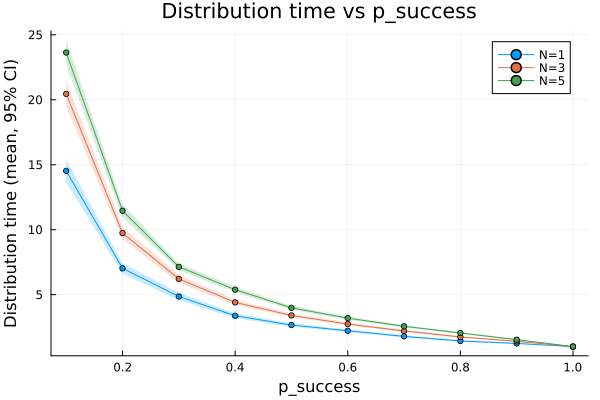
\includegraphics[width=\linewidth]{plot_time_vs_psuccess.png}
    \end{column}
    \begin{column}{0.44\textwidth}
      \textbf{Parameters:} $\pw = 0$, $M = 500$ runs

      \vskip 0.8em
      \begin{itemize}
        \item Time scales as $\sim 1/\ps$ (geometric attempts per link)
        \item Bottleneck: \textbf{slowest link} $T = \max_i T_i$
        \item More repeaters $\Rightarrow$ more links $\Rightarrow$ larger max
        \item Bands: \textbf{95\% CI} of the mean, clipped to $T \geq 1$
      \end{itemize}
    \end{column}
  \end{columns}
\end{frame}

% ============================================================
%  MC SIMULATION - FIDELITY vs p_success
% ============================================================
\begin{frame}{MC Simulation: Fidelity vs $\ps$}
  \begin{columns}[c]
    \begin{column}{0.52\textwidth}
      \centering
      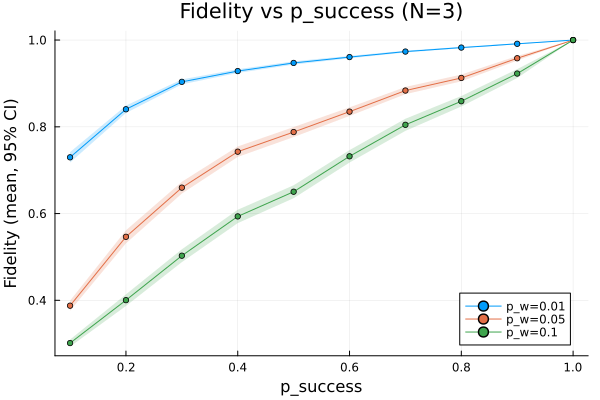
\includegraphics[width=\linewidth]{plot_fidelity_vs_psuccess.png}
    \end{column}
    \begin{column}{0.44\textwidth}
      \textbf{Parameters:} $N = 3$, $M = 500$ runs

      \vskip 0.6em
      {\small
      \begin{itemize}\itemsep0.15em
        \item Low $\ps$ $\to$ long wait $\to$ more depolarization $\to$ $F$ drops
        \item $\pw = 0.10$ degrades far more than $\pw = 0.01$
        \item At $\ps = 1$: $T = 1$ and no inter-link waiting, so $F \to 1$
        \item Bands: \textbf{95\% CI} of the mean, clipped to $[0.25, 1]$
        \item \textbf{Tradeoff:} reliable links reduce both time and degradation
      \end{itemize}}
    \end{column}
  \end{columns}
\end{frame}

% ============================================================
%  MC SIMULATION - FIDELITY vs N
% ============================================================
\begin{frame}{MC Simulation: Fidelity vs $N$}
  \begin{columns}[c]
    \begin{column}{0.52\textwidth}
      \centering
      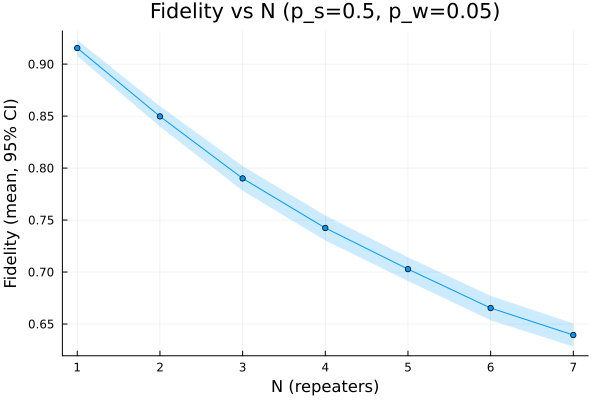
\includegraphics[width=\linewidth]{plot_fidelity_vs_N.png}
    \end{column}
    \begin{column}{0.44\textwidth}
      \textbf{Parameters:} $\ps = 0.5$, $\pw = 0.05$, $M = 500$

      \vskip 0.8em
      \begin{itemize}
        \item $F$ \textbf{decreases monotonically} with $N$
        \item Two effects: more noisy qubits + larger $T = \max_i T_i$
        \item $F \approx 0.92$ ($N\!=\!1$) to $F \approx 0.64$ ($N\!=\!7$)
        \item Asynchronous swaps keep $F$ well above a synchronous bound
        \item Bands: \textbf{95\% CI} of the mean (widen slightly with $N$)
      \end{itemize}
    \end{column}
  \end{columns}
\end{frame}

% ============================================================
%  MC SIMULATION - HEATMAP
% ============================================================
\begin{frame}{MC Simulation: Fidelity Heatmap}
  \begin{columns}[c]
    \begin{column}{0.52\textwidth}
      \centering
      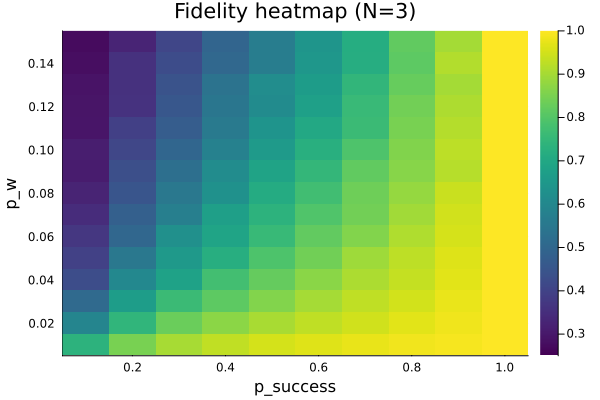
\includegraphics[width=\linewidth]{plot_heatmap_fidelity.png}
    \end{column}
    \begin{column}{0.44\textwidth}
      \textbf{Parameters:} $N = 3$, $M = 500$

      \vskip 0.6em
      2D mean fidelity in $(\ps, \pw)$ space.

      \vskip 0.4em
      {\small
      \begin{itemize}\itemsep0.15em
        \item \textbf{Bottom-right} (yellow): high $\ps$, low $\pw$ $\Rightarrow$ $F \to 1$
        \item \textbf{Top-left} (purple): low $\ps$, high $\pw$ $\Rightarrow$ $F \to 0.25$ (maximally mixed)
        \item Gradient shows \textbf{non-linearity}: at low $\ps$ the waiting time amplifies memory noise
        \item Right edge: $F = 1$ for every $\pw$ (zero waiting time)
      \end{itemize}}
    \end{column}
  \end{columns}
\end{frame}

% ============================================================
%  THEORETICAL FRAMEWORK
% ============================================================
\begin{frame}{Theoretical Framework}
  \begin{columns}[T]
    \begin{column}{0.48\textwidth}
      \begin{block}{Distribution Time}
        \small
        For $N+1$ i.i.d.\ links with $T_i \sim \mathrm{Geom}(\ps)$:
        \[
          \mathbb{E}[T] = \sum_{t=0}^{\infty} \left[1 - \big(1 - (1-\ps)^t\big)^{N+1}\right]
        \]

        \vskip 0.1em
        Harmonic approximation:
        \[
          \mathbb{E}[T] \approx \frac{H(N+1)}{\ps}, \quad H(n) = \sum_{k=1}^n \frac{1}{k}
        \]
      \end{block}
    \end{column}
    \begin{column}{0.48\textwidth}
      \begin{block}{Werner Model (asynchronous)}
        \small
        Depolarized links are Werner states; each qubit survives
        $(1-\pw)^{\Delta}$ over \emph{its own} wait. A repeater qubit is measured
        at its local swap time $\max(T_{i-1}, T_i)$, the end qubits only at $T$:
        \vspace{-0.2em}
        \[
          w_i = (1-\pw)^{\,\Delta^{\mathrm{L}}_i + \Delta^{\mathrm{R}}_i}, \qquad
          \Delta^{\mathrm{L}}_i,\Delta^{\mathrm{R}}_i \le T - T_i
        \]
        Ideal BSMs multiply the Werner parameters:
        \vspace{-0.2em}
        \[
          w_{\mathrm{tot}} = \prod_{i=1}^{N+1} w_i, \quad F = \frac{1 + 3\, w_{\mathrm{tot}}}{4}
        \]
        \alert{Per-qubit} waits $\Rightarrow$ higher $F$ than a synchronous
        schedule (all qubits waiting $T - T_i$).
      \end{block}
    \end{column}
  \end{columns}
\end{frame}

% ============================================================
%  ANALYSIS: TIME COMPARISON
% ============================================================
\begin{frame}{Analysis: MC Time vs Theory}
  \begin{columns}[c]
    \begin{column}{0.55\textwidth}
      \centering
      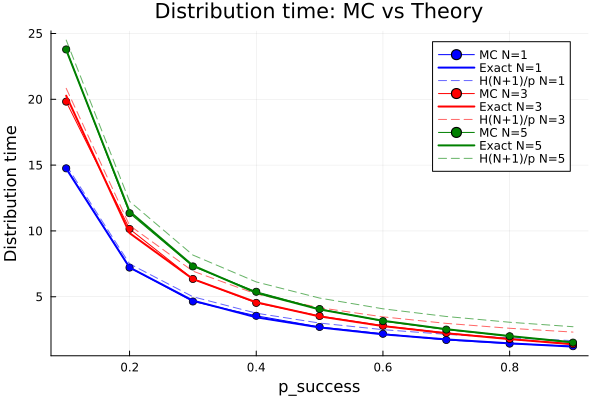
\includegraphics[width=\linewidth]{analysis_time_comparison.png}
    \end{column}
    \begin{column}{0.42\textwidth}
      \begin{itemize}
        \item MC data closely follow \textbf{exact curves} (errors $< 5\%$, $M = 1000$)
        \item Harmonic approx.\ $H(N\!+\!1)/\ps$ accurate at \textbf{low} $\ps$
          (geometric $\to$ exponential limit), overestimates at high $\ps$
        \item Exact formula captures order statistics of i.i.d.\ geometric RVs
        \item Log growth with $N$: see appendix
      \end{itemize}
    \end{column}
  \end{columns}
\end{frame}

% ============================================================
%  ANALYSIS: FIDELITY COMPARISON
% ============================================================
\begin{frame}{Analysis: MC Fidelity vs Werner (async vs synchronous)}
  \centering
  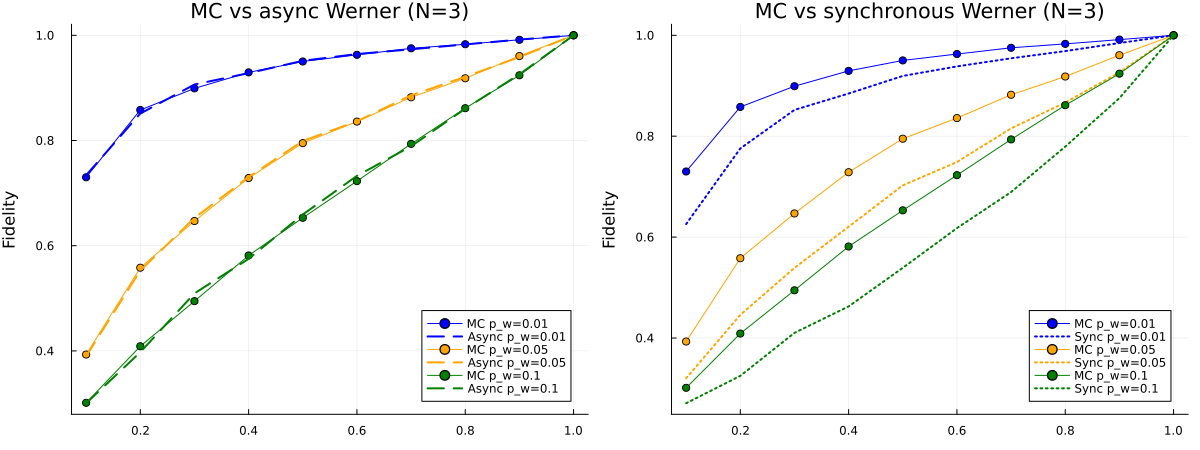
\includegraphics[width=0.80\linewidth]{analysis_fidelity_comparison.png}

  \vskip 0.3em
  \begin{columns}[T]
    \begin{column}{0.45\textwidth}
      \small
      \textbf{Left:} the \alert{asynchronous} per-qubit Werner model matches the
      discrete-event Monte Carlo within statistical error (overlapping 95\% CIs)
      at every $\ps$ and $\pw$.
    \end{column}
    \begin{column}{0.45\textwidth}
      \small
      \textbf{Right:} the \alert{synchronous} schedule (all BSMs at $T$, the
      earlier model) systematically \emph{underestimates} $F$ for $N \ge 2$.
    \end{column}
  \end{columns}
\end{frame}

% ============================================================
%  ANALYSIS: SCALING WITH N
% ============================================================
\begin{frame}{Analysis: Fidelity Scaling with $N$}
  \begin{columns}[c]
    \begin{column}{0.52\textwidth}
      \centering
      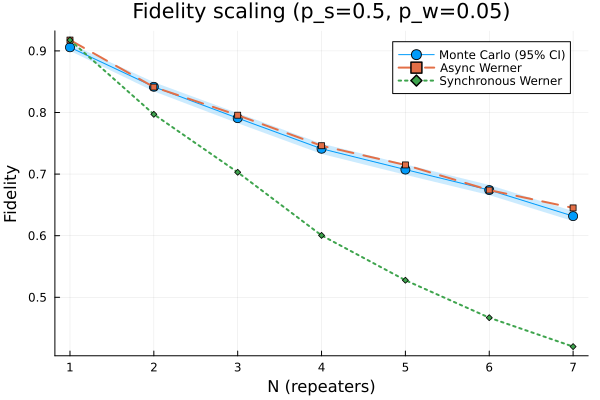
\includegraphics[width=\linewidth]{analysis_scaling_N.png}
    \end{column}
    \begin{column}{0.44\textwidth}
      \textbf{Parameters:} $\ps = 0.5$, $\pw = 0.05$

      \vskip 0.8em
      \begin{itemize}
        \item \textbf{Async} Werner tracks MC at every $N$ (within 95\% CI)
        \item Why: depolarized pairs \emph{are} Werner states; ideal BSMs multiply $w$ exactly
        \item \textbf{Synchronous} Werner falls away for $N \ge 2$: the gap grows to $\sim 0.21$ at $N = 7$
        \item The two coincide at $N = 1$ (no internal qubit is freed early)
      \end{itemize}
    \end{column}
  \end{columns}
\end{frame}

% ============================================================
%  EMERGENT EFFECTS
% ============================================================
\begin{frame}{Emergent Effects}
  \centering
  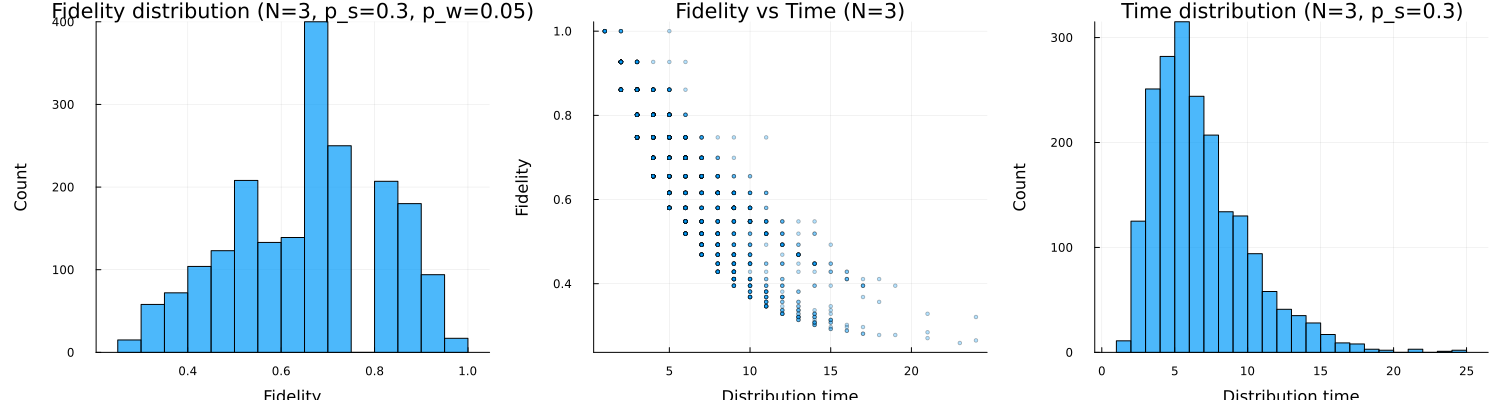
\includegraphics[width=0.88\linewidth]{analysis_emergent.png}

  \vskip 0.3em
  \begin{columns}[T]
    \begin{column}{0.30\textwidth}
      \small
      \textbf{Distribution of $F$:} broad, left-skewed mass down to
      $0.25$ (mixed state); the spikes are the \emph{discrete} values of $F$.
    \end{column}
    \begin{column}{0.34\textwidth}
      \small
      \textbf{$F$ vs $T$:} clear \alert{negative correlation};
      horizontal bands: $F$ is set by the integer waits $T - T_i$,
      so it is \emph{discrete} and still varies at fixed $T$.
    \end{column}
    \begin{column}{0.30\textwidth}
      \small
      \textbf{Distribution of $T$:} right-skewed with a geometric
      (exponential) tail, outliers wait much longer.
    \end{column}
  \end{columns}
\end{frame}

% ============================================================
%  CONCLUSIONS
% ============================================================
\begin{frame}{Conclusions}
  \begin{columns}[T]
    \begin{column}{0.48\textwidth}
      \begin{block}{Main Results}
        \vspace{-0.2em}
        \begin{itemize}\itemsep0.15em
          \item Built on the \textbf{discrete-event} engine: \texttt{ProtocolZoo} entities run in parallel
          \item Swapping preserves $\phiplus$ perfectly (\textbf{validated} $N = 1 \ldots 5$, $T = 1$)
          \item $F$ degrades with $N$, $\pw$, low $\ps$ (noise + waiting time)
          \item \textbf{Async} per-qubit Werner matches MC; the synchronous schedule underestimates $F$ for $N \ge 2$
        \end{itemize}
        \vspace{-0.2em}
      \end{block}
    \end{column}
    \begin{column}{0.48\textwidth}
      \begin{block}{Future Work}
        \vspace{-0.3em}
        \begin{itemize}\itemsep0.05em
          \item Entanglement purification to improve $F$
          \item Classical-communication \textbf{latency} + cutoff times (\texttt{CutoffProt})
          \item Non-linear topologies (trees, graphs)
          \item More realistic noise models (dephasing, losses)
        \end{itemize}
        \vspace{-0.3em}
      \end{block}

      \vskip 0.2em
      \begin{alertblock}{Code}
        \vspace{-0.2em}
        \centering
        \footnotesize\texttt{run\_ideal.jl} $\mid$ \texttt{run\_simulation.jl} $\mid$ \texttt{run\_analysis.jl}
        \vspace{-0.2em}
      \end{alertblock}
    \end{column}
  \end{columns}
\end{frame}

% ============================================================
%  APPENDIX
% ============================================================
\appendix

\begin{frame}[plain, noframenumbering]
  \begin{tikzpicture}[remember picture, overlay]
    \fill[qDark] (current page.north west) rectangle (current page.south east);
  \end{tikzpicture}
  \centering
  \vfill
  {\color{white}\Huge\bfseries Thank You}\\[1em]
  {\color{qCyan}\large Questions?}
  \vfill
\end{frame}

\begin{frame}[noframenumbering]{Appendix: Simulation Parameters}
  \centering
  \small
  \renewcommand{\arraystretch}{1.4}
  \begin{tabular}{l p{3.2cm} p{6.0cm}}
    \toprule
    \textbf{Parameter} & \textbf{Values} & \textbf{Description} \\
    \midrule
    $N$ & $1, 3, 5$ (sim.) / $1$--$7$ (analysis) & Number of repeaters in the chain \\
    $\ps$ & $0.1$--$1.0$, step $0.1$ & Bell pair generation success probability \\
    $\pw$ & $0.01, 0.05, 0.10$ & Per-time-step depolarization parameter \\
    $M$ & $500$ (sim.) / $1000$--$2000$ (analysis) & Number of Monte Carlo iterations \\
    $\tau$ & $-1/\ln(1 - \pw)$ & Depolarization time (QuantumSavory) \\
    attempt & $1.0$ & Duration of one heralded-generation window (= 1 step) \\
    delay & $10^{-9}$ & Classical-channel latency (kept negligible) \\
    bands & $95\%$ CI & Confidence interval of the mean ($1.96\,s/\sqrt{M}$) \\
    Seed & $2025$ & Global RNG seed (reproducible figures) \\
    \bottomrule
  \end{tabular}
\end{frame}

\begin{frame}[noframenumbering]{Appendix: Time Scaling with $N$}
  \begin{columns}[c]
    \begin{column}{0.52\textwidth}
      \centering
      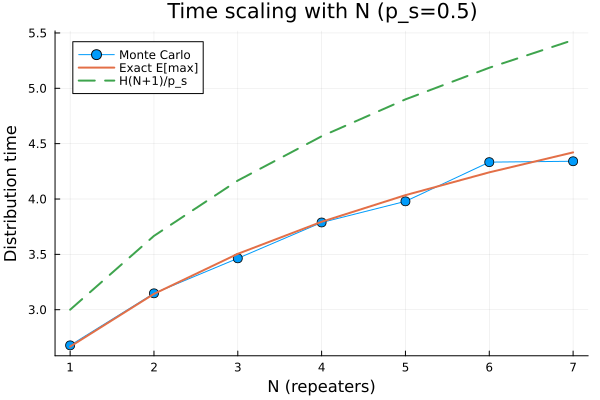
\includegraphics[width=\linewidth]{analysis_time_vs_N.png}
    \end{column}
    \begin{column}{0.44\textwidth}
      \textbf{Parameters:} $\ps = 0.5$, $\pw = 0$, $M = 1000$

      \vskip 0.8em
      \begin{itemize}
        \item $\mathbb{E}[T] = \mathbb{E}[\max_{i \le N+1} T_i]$ grows \textbf{logarithmically} in $N$
        \item Harmonic approximation $H(N\!+\!1)/\ps$ overestimates slightly at moderate $\ps$
        \item Doubling the chain adds little latency --- waiting is dominated by $1/\ps$
      \end{itemize}
    \end{column}
  \end{columns}
\end{frame}

\end{document}
